% Created 2018-06-25 Mon 13:08
% Intended LaTeX compiler: pdflatex
\documentclass[a4paper, oneside]{article}
\usepackage[utf8]{inputenc}
\usepackage[T1]{fontenc}
\usepackage{graphicx}
\usepackage{grffile}
\usepackage{longtable}
\usepackage{wrapfig}
\usepackage{rotating}
\usepackage[normalem]{ulem}
\usepackage{amsmath}
\usepackage{textcomp}
\usepackage{amssymb}
\usepackage{capt-of}
\usepackage{hyperref}
\hypersetup{colorlinks=true, linkcolor=blue}
\usepackage[, frenchb]{babel}
\usepackage[T1]{fontenc}
\usepackage[utf8]{inputenc}
\usepackage{minitoc}
\usepackage{parskip}
\date{\today}
\title{}
\hypersetup{
 pdfauthor={},
 pdftitle={},
 pdfkeywords={},
 pdfsubject={},
 pdfcreator={Emacs 25.3.1 (Org mode 9.1.6)},
 pdflang={Frenchb}}
\begin{document}


\begin{titlepage}

\newcommand{\HRule}{\rule{\linewidth}{0.5mm}} % Defines a new command for the horizontal lines, change thickness here

\center % Center everything on the page

%----------------------------------------------------------------------------------------
%	HEADING SECTIONS
%----------------------------------------------------------------------------------------

\textsc{\LARGE IDEC}\\[1.5cm] % Name of your university/college
\textsc{\Large Projet de fin de 1\up{ère} année}\\[0.5cm] % Major heading such as course name
%\textsc{\large Cahier des charges}\\[0.5cm] % Minor heading such as course title

%----------------------------------------------------------------------------------------
%	TITLE SECTION
%----------------------------------------------------------------------------------------

\HRule \\[0.4cm]
{ \huge \bfseries Générateur de templates \LaTeX{}}\\[0.4cm] % Title of your document
\HRule \\[1.5cm]

%----------------------------------------------------------------------------------------
%	AUTHOR SECTION
%----------------------------------------------------------------------------------------

\begin{minipage}{\textwidth}
\begin{center} \large
Thierry \textsc{Raeber} % Your name
\end{center}
\end{minipage}\\[4cm]
% ~
% \begin{minipage}{0.4\textwidth}
% \begin{flushright} \large
% %\emph{Supervisor:} \\
% %Dr. James \textsc{Smith} % Supervisor's Name
% \end{flushright}
% \end{minipage}\\[4cm]

% If you don't want a supervisor, uncomment the two lines below and remove the section above
%\Large \emph{Author:}\\
%John \textsc{Smith}\\[3cm] % Your name

%----------------------------------------------------------------------------------------
%	DATE SECTION
%----------------------------------------------------------------------------------------

{\large \today}\\[3cm] % Date, change the \today to a set date if you want to be precise

%----------------------------------------------------------------------------------------
%	LOGO SECTION
%----------------------------------------------------------------------------------------

%\includegraphics{Logo}\\[1cm] % Include a department/university logo - this will require the graphicx package

%----------------------------------------------------------------------------------------

\vfill % Fill the rest of the page with whitespace

\end{titlepage}
\tableofcontents
\pagebreak

\part{Manuel utilisateur}
\section{Fenêtre de gestion principale}
\label{sec:orgbec1e98}

Au lancement du programme, celui-ci se présente comme illustré par la figure \ref{fig:org5289734}.

\begin{figure}[htbp]
\centering
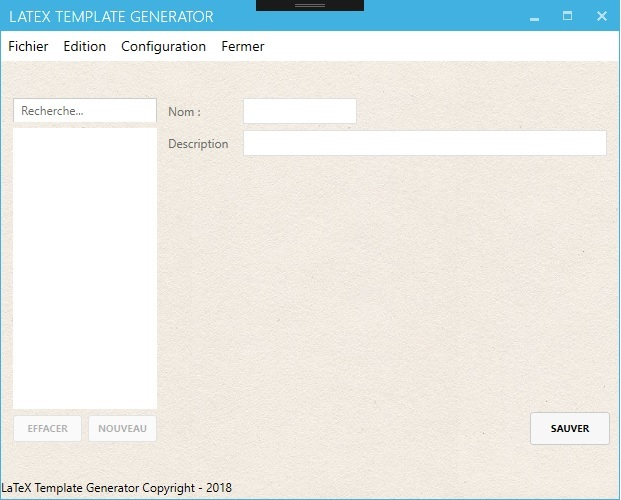
\includegraphics[width=.9\linewidth]{../Images/accueil.jpg}
\caption{\label{fig:org5289734}
Fenêtre principale (vide)}
\end{figure}

Cette fenêtre présente la structure commune à toutes les fenêtres de gestion,
que ce soit la gestion des templates, des macros, des environnements ou des
meta-packages. Comme rien n'est sélectionné, tout est grisé.

\subsection{Gestion des templates}
\label{sec:org714228c}
Le menu "Edition" permet de choisir le type d'élément à gérer. Ainsi, la fenêtre
de gestion des templates est illustré par la figure \ref{fig:org0beb42d}.
\begin{figure}[htbp]
\centering
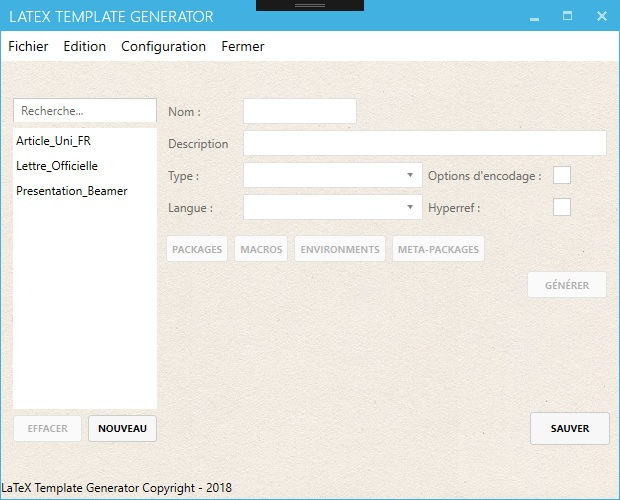
\includegraphics[width=.9\linewidth]{../Images/template_vide.jpg}
\caption{\label{fig:org0beb42d}
Fenêtre de gestion des templates (vide)}
\end{figure}

On constate d'une part que la liste de gauche a été populée avec les templates
présents dans la base de donnée. De plus, en plus des champs "Nom" et
"Description" déjà présents sur l'interface, un certain nombre d'éléments ont
été rajoutés. Un template doit en effet également avoir un "type" (article,
book, letter, etc). On lui attribue également une langue qui permet de définir
l'hyphénation, certains caractères spéciaux, les règles typographiques
spécifiques à une langue donnée, comme la forme des guillemets, etc. On a
ensuite le choix d'ajouter les options d'encodage pour formatter son document en
UTF-8 (cette option est activée par défaut), et finalement, d'ajouter ou non le
package \emph{hyperref}. Ce dernier sert à gérer les liens hypertexte. Or il a la
particularité de devoir être toujours placé en dernier, après tous les autres
packages. Cette gestion indépendante des autres packages rendait son intégration
plus aisée.

On observe également qu'un ligne de boutons "Packages", "Macros",
"Environements", "Meta-packages" est apparue. Cette ligne reviendra dans chacune
des fenêtre de gestion pour les autres entités, et permet la gestion des
\emph{dépendances}. Nous y revenons au \hyperref[orge9adf42]{chapitre} \ref{orge9adf42}.


Finalement, un bouton "Générer" est également présent, qui servira à présenter
le code final, que nous décrivons au \hyperref[org28f775d]{chapitre}  \ref{org28f775d}

A noter que tant qu'aucun template n'est sélectionné, presque tout est
grisé. Seul le bouton "Nouveau" (et le bouton "Sauver" mais ça doit être
corrigé) est disponible, car il ne nécessite pas qu'un élément soit
sélectionné. Une fois qu'on a sélectionné un template, tout se déverrouille,
comme le montre la figure \ref{fig:org4be422c}.

\begin{figure}[htbp]
\centering
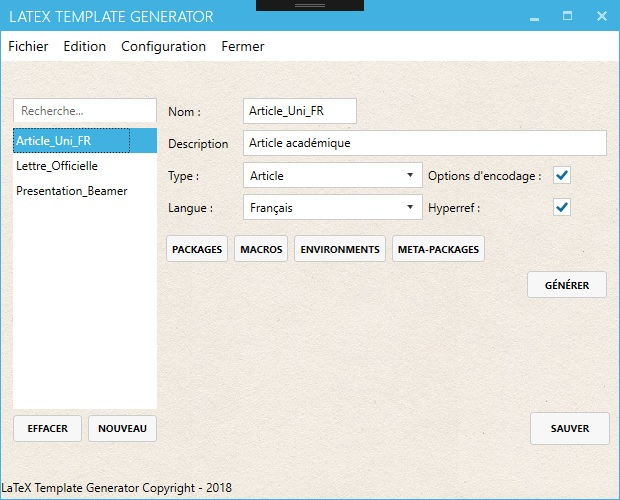
\includegraphics[width=.9\linewidth]{../Images/template_full.jpg}
\caption{\label{fig:org4be422c}
Fenêtre de gestion des templates}
\end{figure}

\subsection{Gestion des macros}
\label{sec:org6e52093}

La fenêtre des macros est très similaire avec la figure \ref{fig:org2401d34}.

\begin{figure}[htbp]
\centering
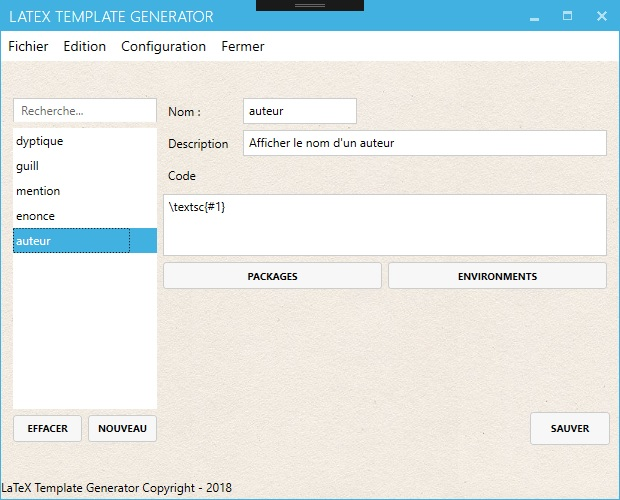
\includegraphics[width=.9\linewidth]{../Images/macro.jpg}
\caption{\label{fig:org2401d34}
Fenêtre de gestion des macros}
\end{figure}

Elle ne possède comme champ propre que le champ "Code", qui permet de définir le
contenu de la macro dans le document final.

Elle n'intègre par ailleurs que les boutons "Package" et "Environement", les
autres n'étant pas nécessaires. En effet, selon ce design, une macro ne peut
avoir comme dépendance une autre macro, ou un méta-package.

A noter que le bouton "Générer" a également disparu, car il ne peut être associé
qu'avec un template.

\subsection{Gestion des environements}
\label{sec:org52b7968}

Très similaire à la fenêtre de gestion des macros, celle des environnements est
illustrée par la figure \ref{fig:org113a461}.

\begin{figure}[htbp]
\centering
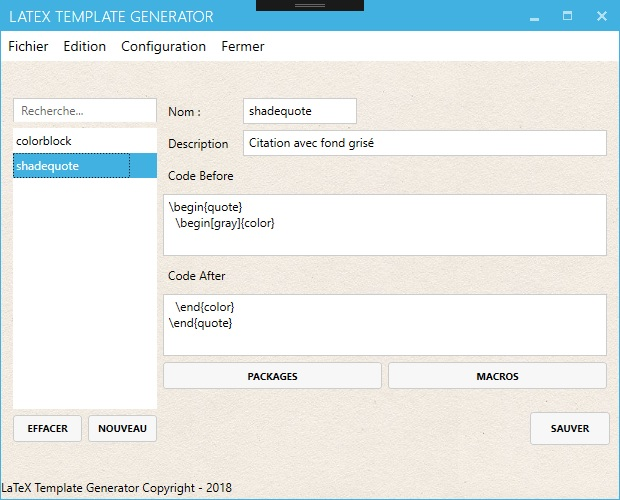
\includegraphics[width=.9\linewidth]{../Images/environment.jpg}
\caption{\label{fig:org113a461}
Fenêtre de gestion des environements.}
\end{figure}

On retrouve la plupart des champs précédents. Toutefois, un environnement est
défini par le code initial, et le code final. Le reste est très similaire à ce
qu'on a vu jusque là.

\subsection{Gestion des méta-packages}
\label{sec:orgfe6e7b7}

La gestion des méta-packages est encore plus simple, comme le montre la figure \ref{fig:orgd87d7a9}.

\begin{figure}[htbp]
\centering
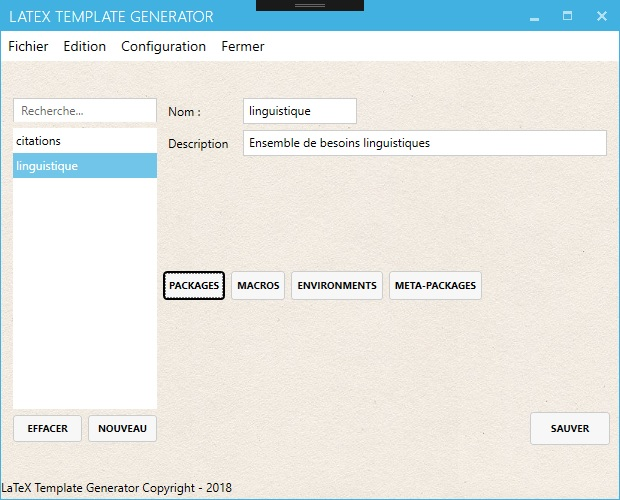
\includegraphics[width=.9\linewidth]{../Images/meta.jpg}
\caption{\label{fig:orgd87d7a9}
Fenêtre de génération du code}
\end{figure}

Puisqu'un méta-package ne possède aucun code propre, mais n'est qu'un
regroupement d'éléments sous une même fonctionnalité, il n'implémente qu'une
gestion des dépendances pour tous les types d'objets : packages, macros,
environnements et méta-packages (un méta-package pour appeler un autre
méta-package).

\section{Fenêtre de gestion des dépendances}
\label{sec:orgbe7d198}
\label{orge9adf42}

Nous allons expliquer ici ce qui apparaît lorsqu'on clique sur les boutons de
gestion des dépendances. En effet, une entité (un template, une macro, etc) peut
nécessité l'intégration d'autres éléments pour être fonctionnelle. Chaque
fenêtre de gestion offre donc les boutons permettant d'ouvrir la boite de
gestion des dépendances. Celle-ci fonctionne de manière identique pour tous les
type d'objets, nous n'en décriront donc qu'une seule. Sa forme est illustrée par
la figure \ref{fig:orga7d6348}.

\begin{figure}[htbp]
\centering
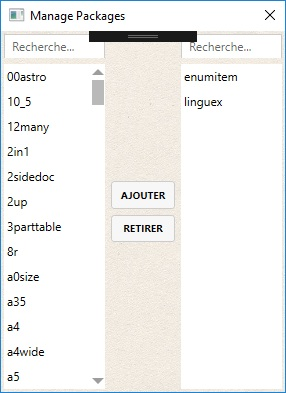
\includegraphics[width=200px]{../Images/packages.jpg}
\caption{\label{fig:orga7d6348}
Fenêtre de gestion des dépendances}
\end{figure}

La liste de gauche présente l'ensemble des éléments disponibles (ici,
les \(\sim\)10'000
packages), dont on peut réduire le nombre grâce au champ de recherche. La liste
de droite présente les éléments inclus dans la relation de dépendance avec
l'item préalablement sélectionné dans la fenêtre parente.

Sélectionner un item dans la colonne de gauche et cliquer "Ajouter" permet de le
placer dans la colonne de droite. Sélectionner un item dans la colonne de droite
et cliquer "Retirer" permet de l'enlever. Pour éviter les problèmes,
sélectionner un item dans une colonne dé-sélectionne automatiquement l'item de
l'autre colonne.

\section{Fenêtre de code généré}
\label{sec:orgf3f4103}
\label{org28f775d}

La fenêtre de génération du code \LaTeX{} final est représenté par la figure \ref{fig:org1d1fae8}.
\begin{figure}[htbp]
\centering
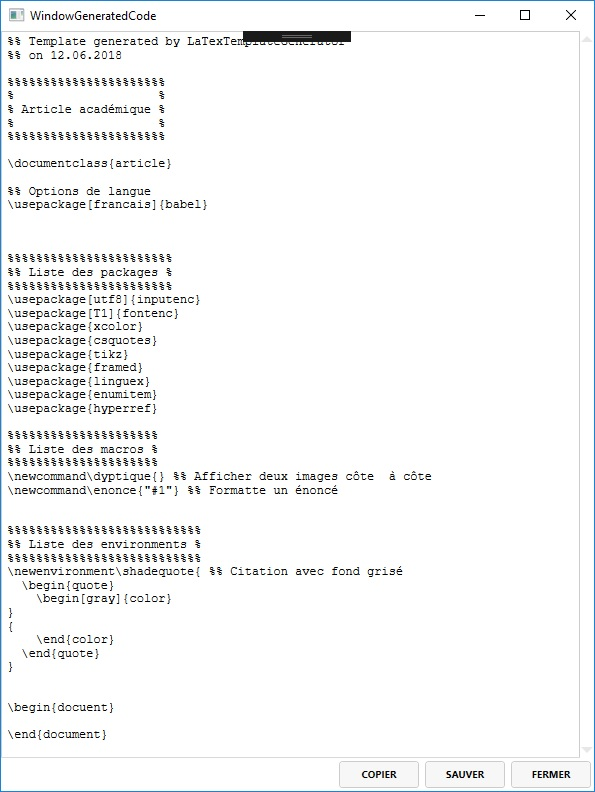
\includegraphics[width=.9\linewidth]{../Images/code.jpg}
\caption{\label{fig:org1d1fae8}
Fenêtre de génération du code}
\end{figure}

Cette fenêtre contient une textbox non éditable contenant l'ensemble du code
généré. Un bouton "Copier" permet de copier le contenu du code dans le
presse-papiers. Un bouton "Sauver" permet de sauver le code directement dans un
fichier .tex, et un bouton "Fermer" permet de fermer la fenêtre.

\section{Fenêtre de gestion des packages}
\label{sec:org033edce}
La fenêtre de gestion des packages se présente comme illustré par la
figure \ref{fig:orgd9f5077}.
\begin{figure}[htbp]
\centering
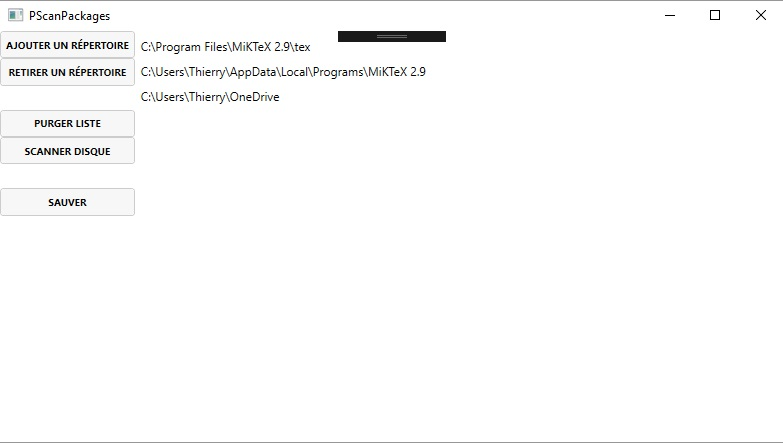
\includegraphics[width=.9\linewidth]{../Images/scan.jpg}
\caption{\label{fig:orgd9f5077}
Fenêtre de gestion des packages}
\end{figure}

Cette fenêtre offre la possibilité d'ajouter / retirer des dossiers à
scanner. Elle offre aussi la possibilité de scanner les dossiers
intégrés à la recherche de nouveaux fichiers .sty. La fonction "Purge"
n'est pas encore implémentée.

\pagebreak
\setcounter{section}{0}
\part{Cahier des charges}


\section{Introduction}
\label{sec:org8fec597}

\LaTeX{} est à la fois un langage et un système de composition de
documents. En substance, \LaTeX{} est à un document écrit ce qu'un
ensemble de plans est à un bâtiment. L'utilisateur écrit le code
source dans un fichier .tex, et ce dernier est lu par un compilateur
qui transforme ce code source en fichier PDF. Le présent cahier des
charges est d'ailleurs rédigé en \LaTeX{}. Le but de ce projet est de
réaliser une application permettant de générer et gérer des templates
de documents \LaTeX{}.

\section{Contexte}
\label{sec:org8c460dd}

Tout document \LaTeX{} est structuré en deux parties distinctes: le préambule,
et le corps. Le corps forme le \emph{contenu} du document, et est délimité par les
balises \texttt{\textbackslash{}begin\{document\}} et \texttt{\textbackslash{}end\{document\}}.  Le préambule est l'ensemble des
instructions qui définissent ce à quoi devra ressembler et se comporter le code
présent dans le code. Si le contenu d'un document change à chaque fois, le
préambule est souvent le même d'un type de document à l'autre, et sa gestion peut
être fastidieuse si elle doit être faite manuellement. Ce logiciel a pour
objectif de faciliter la gestion du préambule d'un document à l'autre.

Plus précisément, un préambule \LaTeX{} est constitué, en simplifié, de 3
composants différents:

\begin{enumerate}
\item les packages
\item les macros personnalisées
\item les environnements personnalisés
\end{enumerate}

Un package est un ajout aux fonctionnalités de bases offertes par \LaTeX{}, un
peu comme un add-on pour Firefox. Il existe des packages quasi systématiquement
ajoutés, comme le package \emph{hyperref} qui gère les liens hypertextes, ou le
package \emph{babel} qui gère les spécificités liées à la langue dans laquelle le
document est rédigé (caractères spéciaux, hyphénation, forme des guillemets,
etc). Il existe également des packages beaucoup plus spécialisés, comme le
package \emph{linguex} qui permet de gérer la numérotation des exemples dans les
textes de linguistique.

Les macros et les environnements sont à voir comme des fonctions en
programmation. Chaque macro ou fonction est invoquée par son nom, et exécute le
code qui lui est associé. La différence est que la macro a la forme \texttt{\textbackslash{}<nom-de-macro>}
, alors que l'environnement apparaît comme une balise qui
s'exécute sur le texte inclus :

\begin{verbatim}
\begin{<nom_de_l'environement>}
Texte sur lequel s'exécutera le code de l'environement.
\end{<nom_de_l'environement>}
\end{verbatim}

Le but de ce logiciel est de faciliter la gestion de ces inclusions.

\section{Objectif}
\label{sec:org02e548f}

Le but de ce programme est de simplifier et automatiser la réalisation
de documents \LaTeX{}. En particulier, l'objectif est d'aider à
générer un préambule en indiquant quels packages et macros
sélectionner.

\section{Fonctionnalités métiers}
\label{sec:org2580d19}
\subsection{Gestion des  templates}
\label{sec:org1bfcbeb}
Un template est un modèle de document type. Ça peut être un article
scientifique, une lettre officielle, un diaporama, etc. Or comme nous l'avons
vu, le préambule d'un document \LaTeX{} est constitué d'un nombre
potentiellement important de packages, de macros et d'environnements. La
fonctionalité principale de ce logiciel sera d'assister l'intégration de ces
différents éléments au sein du préambule. Voici donc la liste des fonctionalités
liées à la gestion des templates, par ordre de priorité d'implémentation:

\subsubsection{Définir un type de document}
\label{sec:orga2f4dc3}
Un document \LaTeX{} est en priorité défini par son type (article, book, letter,
etc). Ceci impactera fortement sur le rendu de mise en page. Il est donc
nécessaire qu'une option définisse ce paramètre. Celui-ci prendra la forme d'une
combobox, car les possibilités de type sont limitées, et fixées d'avance
dans le programme.
\subsubsection{Un bouton "Exporter"}
\label{sec:orgb098c92}
Ce bouton appellera le constructeur du rendu final. Une page
s'ouvrira, dans laquelle apparaît le préambule complet, compilable
tel quel (en théorie). Le texte sera sélectionnable, mais en lecture
seule. L'option "Enregistrer" sauvera le texte dans un fichier au
format .tex. Un bouton "Copier dans le presse-papiers" sera peut-être
également présent.
\subsubsection{Un bouton "Sauver"}
\label{sec:org4dd5b47}
Ce bouton enregistrera les modifications apportées à template dans la base de
données.
\subsubsection{Choisir les packages, macros et environnements}
\label{sec:org3668976}
Le programme donnera la possibilité de déterminer les différents
packages, macros et environnements désirés. Pour ce faire, un bouton
par type sera présent sur l'interface. Chacun d'eux ouvrira une
nouvelle fenêtre avec à gauche, la liste des éléments disponibles, et
à droite, la liste des éléments prévus pour intégration.
\subsubsection{Choisir la langue du document}
\label{sec:orgb7ad1cb}
Une option pourra être ajoutée pour définir la langue d'édition du document.
\subsubsection{Intégrer le package \emph{hyperref}}
\label{sec:org7d56928}
Une option spécialement dédiée au package hyperref est présente, car
ce package a la particularité de devoir toujours être ajouté en
dernier.
\subsection{Gestion des macros}
\label{sec:org5688fb4}
La fenêtre d'édition des macros offrira une liste recherchable contenant toutes
les macros déjà existantes dans la base de données. Une fois sélectionnée, la
fenêtre affichera le nom de la macro, sa description, ainsi que son code
interne.

la fenêtre permettra également d'effacer une macro existante, ou d'en créer de
nouvelles. Dans un tel cas, les champs se vident, et l'utilisateur pour les
remplir à sa guide.

Les macros peuvent nécessiter la présence de packages préalablement
inclus, ou d'autres macros/environnements préalablement définis. Pour cette
raison, il sera possible de gérer leurs dépendances de la même manière que pour
les templates.
\subsection{Gestion des environnement}
\label{sec:org538abb6}
Étant donné que l'environnement fonctionne de la même manière qu'une macro (seule la
syntaxe de son appel change), il reçoit les mêmes fonctionnalités que la macro.
\subsection{Gestion des meta-package}
\label{sec:org59cdef6}
Un meta-package est un ensemble de packages, de macros et
d'environnements qui sont réunis pour servir un objectif unifié. On
peut imaginer un objectif très minimal, comme "écrire en français",
qui demandera le package \emph{babel} pour l'hyphénation et les guillemets
à chevrons, et le package \emph{fontenc} pour les accents. Rien de
plus. Mais on peut imaginer le bien plus imposant meta-package
"article scientifique en français", qui, en plus du meta-package pour
le français, demandera le meta-package qui gère la bibliographie aux
normes APA, un meta-package gérant les indexes, un meta-package pour
les entêtes et pieds de page, un meta-package pour la table des
matières, etc. Un meta-package peut être vu comme un UserControl en
programmation WPF. C'est une brique formée de briques plus petites,
parfois intégré à une brique de plus haut niveau, et qui finit par
être intégrée dans un template final.

Un meta-package possède un nom, une description, mais pas de code
propre. L'interface de gestion permet de lui attribuer les packages,
macros, et environnements désirés, comme vu précédemment.

\subsection{Gestion de packages}
\label{sec:org9b6d427}
La gestion des packages est plus complexe. Les packages disponibles
sont définis en fonction de l'installation TeXLive faite sur la
machine. Il est donc nécessaire de scanner le disque à la recherche
des fichiers .sty présents. Une interface a donc été crée pour
permettre de
\begin{enumerate}
\item Gérer les dossiers à scanner à la recherche de fichiers .sty
\item Une fonction "Scan" qui opère un scan récursif des dossiers
concernés, et qui ajoute les éventuels packages qui ne sont pas
déjà présent dans la base de donnée
\item Dans le futur, une option "Purge" pourra être implémentée, qui
retire tous les packages non sollicités par les templates, et qui
permet de remettre la base à zéro pour nettoyer les éventuels
packages qui auraient disparus.
\end{enumerate}

\section{Données}
\label{sec:orgbd0f86f}
\subsection{Tables dans la DB}
\label{sec:org7458969}
Tables principales :
\begin{itemize}
\item Package
\item Template
\item Macro
\item Environment
\item meta-package
\item Langue
\item TypeDoc
\item ScanDir
\end{itemize}

A l'exception de la table ScanDir, toutes les autres tables
principales possèdent un champ "Nom" qui permet l'identification de
l'entité par l'utilisateur. Les tables \emph{Template}, \emph{Package}, \emph{Macro},
\emph{Environment} et \emph{Meta} possèdent toutes un champ "Description" qui
permet à l'utilisateur d'insérer une remarque liée à la fonction de
l'entité. Certaines tables, comme la table \emph{Macro} et la table
\emph{Environment} possèdent des champs permettant de définir le code
\LaTeX{} qui constitue leur définition.

\subsection{Schéma}
\label{sec:orgfc4529f}
\begin{figure}[htbp]
\centering
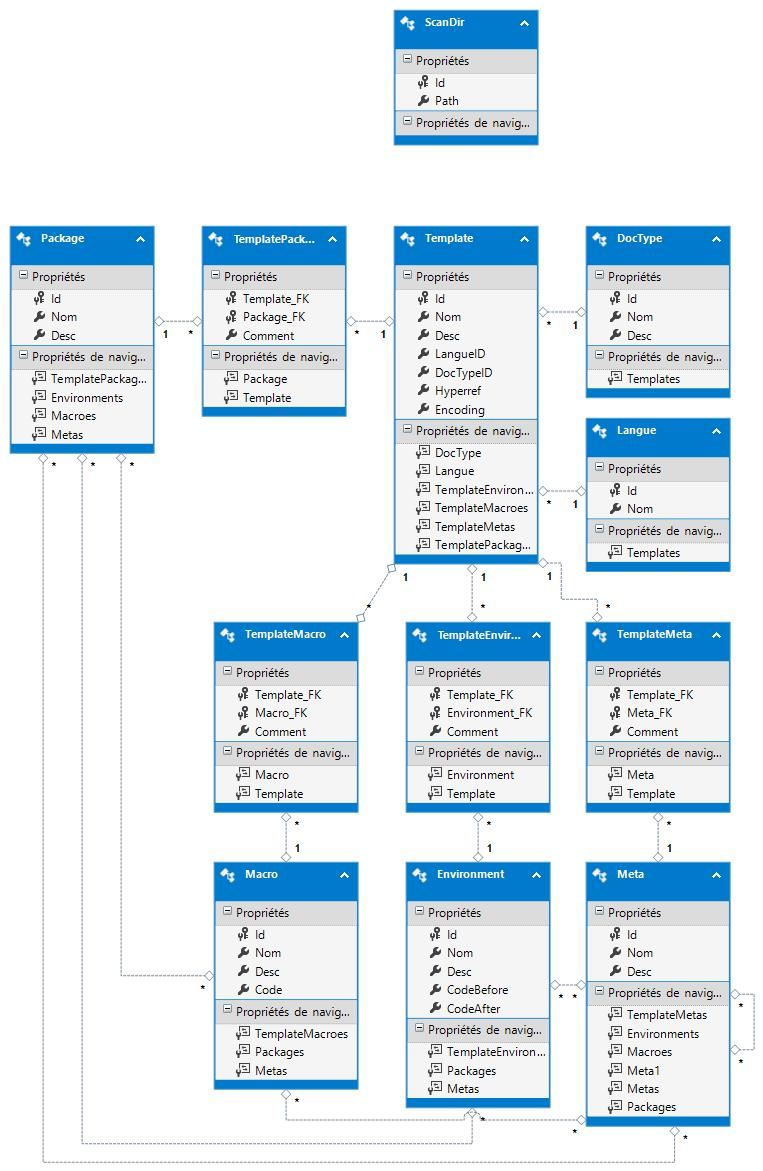
\includegraphics[width=.9\linewidth]{../Images/EntityDesignerDiagram.jpg}
\caption{\label{fig:org2dbedff}
Modèle edmx de la base de données}
\end{figure}

\pagebreak
\setcounter{section}{0}
\part{Documentation technique}


\section{Généralités}
\label{sec:orgd957e06}
Le présent logiciel a été réalisé en C\#, depuis la plateforme de développement
.Net, à l'aide de l'IDE Visual Studio 2017. Il intègre une base de
données réalisée avec SQLServer. L'interface graphique est réalisée en
WPF.


\subsection{Dépendances}
\label{sec:org5391ffa}
Ce logiciel requiert l'installation des plugins NuGets suivants:
\begin{itemize}
\item \emph{EntityFramework}, pour la gestion de la base de données
\item \emph{MahApps.Metro}, pour l'esthétique des fenêtres WPF.
\item \emph{MvvmLight}, qui facilite la communication entre boutons et méthodes
du code-behind.

\textbf{*} Architecture en couches
\end{itemize}
La couche \emph{Données} est implémentée dans le projet "LTG\(_{\text{Entity}}\)". La base
de données est externe, mais le plan edmx et l'ensemble des entités
complétées se trouve dans ce projet. En particulier, les objects de la
base de données qui ont nécessité une classe partielle complétée se
trouvent dans le dossier \emph{Entity}. Quelques requêtes SQL utiles ont
été sauvées dans le dossier \emph{Queries}.

Les couches \emph{Métier} et \emph{Interface} sont toutes deux implémentées dans
le projet "WpfMainView". Toutefois, elles ont été réparties dans des
dossiers séparés. Les éléments d'interface sont répartis en deux
dossier. Le dossier "Controls" contient tous les \emph{UserControls}, et le
dossier "Views" contient toutes les pages et les fenêtres. Concernant
la couche \emph{Métier}, les différents ViewModels sont placés dans le
dossier du même nom, et les différentes classes responsables de tâches
particulières aidant au bon déroulement du programme sont placées dans
le dossier "Helpers".

\section{Base de données}
\label{sec:org2f403bc}
Le schéma edmx de la base de données se présente comme suit:
\begin{figure}[htbp]
\centering
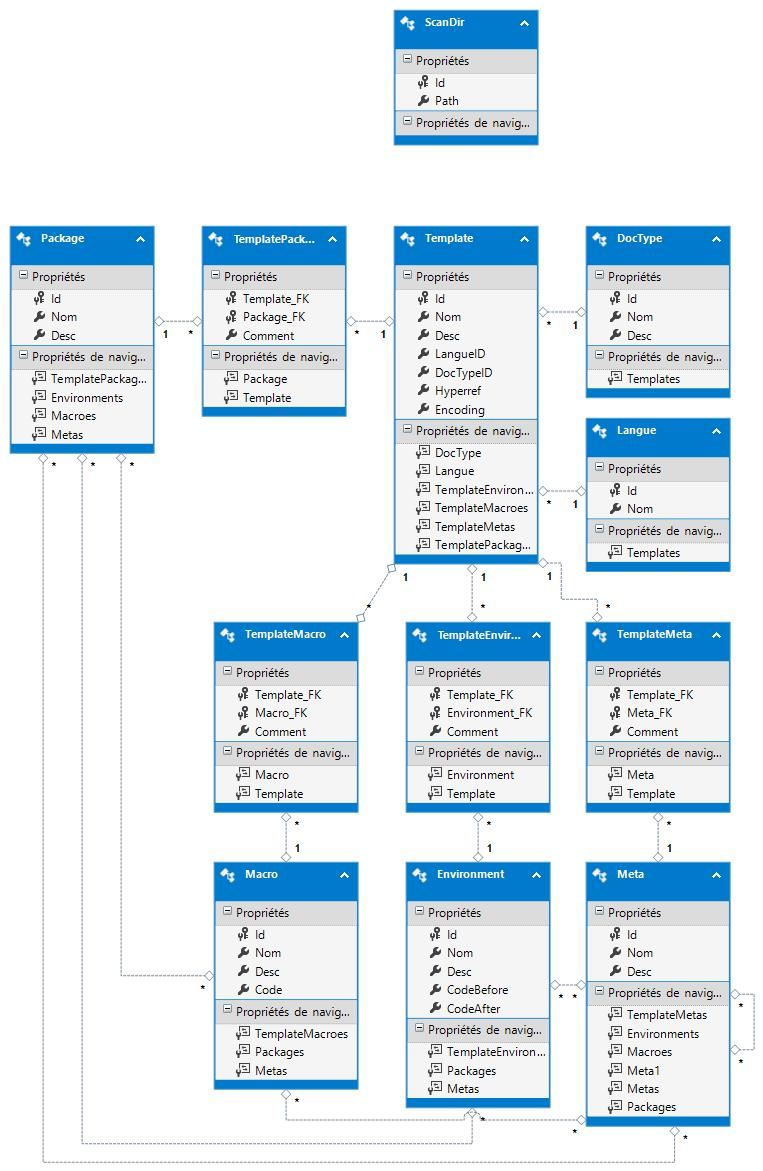
\includegraphics[width=.9\linewidth]{../Images/EntityDesignerDiagram.jpg}
\caption{\label{fig:orgbed741a}
Schéma edmx de la base de données}
\end{figure}

Les entités \emph{Template}, \emph{Macro}, \emph{Meta}, \emph{Environment} et \emph{Package}
entretiennent entre elles des relations n-n. En effet, un template par
exemple peut être associé avec autant de packages qu'on le souhaite, y
compris 0. Ceci explique la présence des tables intermédiaires (comme
TemplatePackage par exemple). A noter que le schéma edmx ne montre pas
les tables intermédiaires lorsque ces tables de contiennent que les
clés étrangères (par économie de place). Pour cette raison, la table
\emph{MetaPackage} par exemple n'apparaissent pas. Toutefois, les tables
liées à l'entité \emph{Template} apparaissent car elles possèdent en propre
un champ \emph{commentaire}, qui servira dans une version ultérieure de ce
programme.

L'entité \emph{Template} entretient également une relation 1-n avec les entités \emph{Langue} et
\emph{DocType} car un template possède obligatoirement 1 et un seul type de
document. Mais un type de document peut être associé à plusieurs
templates. Pareil pour la langue.

Pour finir, l'entité ScanDir n'est reliée à rien, car elle ne sert
qu'à enregistrer les dossier à scanner pour trouver les dossiers .sty.
\subsection{Classes liées aux données}
\label{sec:orgc400bda}
Afin de permettre au programme de proprement caster chacune des listes
de données à afficher, une classe mère \emph{DBItem} est crée. Celle-ci
possède une propriété \emph{Name} qui servira à afficher le nom de l'entité
dans la liste.

Chaque entité principale de la base possède un complément de classe
partiel permettant d'assurer sa bonne gestion. En particulier, chacune
possède une méthode pour créer une nouvelle entité. Cette méthode
contrôle la définition des différents champs. Ceci permet entre autre
de définir à -1 l'ID d'une nouvelle entité, ce qui permet de repérer
chaque entité nouvellement crée, et de l'intégrer proprement à la base
de données.

\section{Classes utilitaires}
\label{sec:org24ac5d0}
Les classes suivantes, localisées dans le dossier "Helpers" du projet
WpfMainView, ont été créées afin de réaliser certaines fonctions
pratiques et récurrentes. Leur fonctionnalité est détaillée ici.

\subsection{La classe Linq()}
\label{sec:org9cc2b21}
La classe Linq sert à regrouper sous une même enseigne des méthodes
liées à l'accès aux données via des commandes Linq. En particulier,
ces méthodes permettent d'obtenir facilement les macros associées à un
template particulier par exemple.

Les méthodes \emph{overloaded} de structure \texttt{DependenciesList(DBItem,
DBItemType)} retournent la liste de dépendances de type \emph{DBItemType}
de l'objet \emph{DBItem} passé en paramètre.

Les méthodes de structure \texttt{List*(DBItem)} (ListPackages par exemple)
retournent également une liste de dépendances de l'objet passé en
paramètre, et dont le type est défini par le nom. Contrairement aux
méthodes de type DependenciesList, celles-ci retournent une liste de
type correspondant au nom de la méthode, et non une liste de DBItems

Les méthodes \emph{overloaded} de structure \texttt{RemoveJoin(DBItem, DBItem)}
servent à retirer le lien potentiellement existant dans la base de
donnée entre les deux entités. Ces méthodes sont en particulier
utilisées lors de la destruction d'un objet, pour s'assurer que toutes
les connexions intermédiaires sont également détruites.


Étant donné que ces méthodes ne sont là que pour offrir de manière
plus aisée accès à certaines procédures Linq, elles sont toutes
statiques.
\subsection{La classe PackageScan()}
\label{sec:orgc588356}
Cette classe sert à gérer le scan du disque à la recherches de
nouveaux .sty. Pour l'instant, elle ne contient que la méthode
\texttt{StyFromDir(string Dir)} qui retourne une liste de strings
correspondant au nom de tous les fichiers .sty trouvés dans le dossier
passé en paramètre. Dans le futur, elle pourrait accueillir d'autres
méthodes, comme le retrait de packages non utilisés par exemple, ou la
gestion des dossiers eux-mêmes, qui pour l'instant sont gérés
ailleurs.
\subsection{La classe TemplateContent()}
\label{sec:org3067a49}
Cette classe stocke et gère toutes les informations nécessaires au
formattage d'un template en code \LaTeX{}. Elle n'implémente qu'un
seul constructeur, qui reçoit un template en paramètre. Le
constructeur fixe certaines informations et appelle ensuite la
fonction \texttt{ComputeContent()} qui s'occupe de récupérer l'ensemble des
packages, macros, environnements et méta-packages passés en dépendance
préalablement.

Les méthodes \emph{overloaded} de structure \texttt{Add(DBItem)} gèrent
l'intégration des informations liées à l'item passé en paramètre. Par
exemple, si une macro en paramètre, la fonction \texttt{Add(Macro m)}
s'assure d'une part que la macro est bien ajoutée à la liste, mais que
tous les packages dont elle dépend sont également ajoutés. Pareille
pour un environnement. La méthode \texttt{Add(Meta m)} s'assure que tous les
packages, tous les environnements et toutes les macros associées sont
ajoutés, mais également tous les métas-packages qui pourraient y être
associés également. Pour éviter tout problème de circularité infinie,
un item est tout d'abord ajouté à la liste finale, avant de vérifier
ses dépendances. Ceci permet que dans un cas où le méta-package A
inclut le méta-package B qui inclut le méta-package C qui lui-même
inclut le méta-package A, chacun des méta-packages n'est contrôlé
qu'une seule fois.

La méthode \texttt{ComputeContent()} appelle donc simplement la méthode
\texttt{Add()} sur toutes les dépendances directes du template. Ce sont les
méthodes \texttt{Add()} elles-mêmes qui s'occuperont de retrouver les
dépendances récursives.
\subsection{La classe TemplateFormatter()}
\label{sec:org16e92bb}
La classe \texttt{TemplateFormatter()} sert à générer le code \LaTeX{}
final. L'unique constructeur de cette classe prend un objet de type
TemplateContent en paramètre. Celui-ci contient la liste exhaustive de
tous les éléments associés au template. Il suffit donc de les prendre
dans l'ordre, et de les transformer en texte proprement formatté.

Les méthodes de type \texttt{ToLatex()} prennent soit un package, soit une
macro, soit un environnement, et retournent un string correspondant au
code \LaTeX{} de leur définition / inclusion. Leur contenu est peu
intéressant, et consiste simplement à respecter les règles de syntaxe
du langage \TeX{}.

La méthode \texttt{generate()} appelle les unes après les autres les méthodes
nécessaires au bon formattage du document final. A noter simplement
que les entêtes de type "Liste des macros" n'apparaissent que si le
nombre de macros est non nul. La méthode retourne un string
correspondant au code complet du template.
\subsection{La classe VMHelper}
\label{sec:org5a0d808}
Cette petite classe  contient une énumération qui a été crée
pour permettre de déterminer plus facilement de quel type de donnée
l'utilisateur est en train de gérer. Elle implémente également une
méthode retournant la liste d'items de la base de donnée en fonction
du type passé en paramètre.
\section{Interface graphique}
\label{sec:org0f55c6e}
Les fenêtres se trouvent toutes dans le dossier "Views". Les
UserControls se trouvent dans le dossier "Controls".

Une grande partie des UserControls qui ont été développés ne sont
finalement pas utilisés. En effet, je ne suis pas parvenu à
correctement connecter les données entre les ViewModels et les
UserControls pour parvenir à mes fins. Je ne maîtrise pas encore assez
la gestion des DataContexts. J'ai donc du me résigner à répéter le
code en question, ce qui est totalement non-optimal. Mais ça
marche. Désolé.

\subsection{Les fenêtres}
\label{sec:org14b8b03}
\subsubsection{Fenêtre principale}
\label{sec:orgd34ba8d}
La fenêtre principale, sur laquelle on arrive au lancement du
programme, est implémentée dans le fichier "MainWindow.xaml". Cette
fenêtre implémente simplement un menu en haut, une barre
d'informations en bas, et un espace pour contenir le UserControl
implémenté dans le fichier "UCManager.xaml". Il serait idéalement
préférable de fondre le UserControl \emph{UCManager} directement dans la
fenêtre \emph{MainWindow}. Toutefois, faire cela requiert de modifier les
ViewModels associés, ce qui prendrait trop de temps. J'ai donc décidé
de laisser les choses ainsi pour l'instant.

\subsubsection{Fenêtre de gestion des dépendances}
\label{sec:orga7af3b4}
La fenêtre de gestion des dépendances est implémentée dans le fichier
"PManageDependencies.xaml". Elle est constituée de deux listes à
gauche et à droite, et de deux boutons au centre.

\subsubsection{Fenêtre de gestion des packages}
\label{sec:orgcfbc3e1}
La fenêtre de gestion des packages est implémentée dans le ficher
"PScanPackages.xaml". J'avoue qu'elle est assez moche, vu qu'elle a
été implémentée tout à la fin.

\subsection{Les UserControls}
\label{sec:org8196fae}
Le UserControl le plus important est \emph{UCManager}, dans le fichier du
même nom. Ce UC définit le contrôle principal de gestion des entités
de la base de données. Il contient une colonne à gauche pour afficher
l'ensemble des entités de la liste sélectionnée, et les champs communs
à toutes les entités. Il laisse une grande zone libre en bas à droite
pour afficher les particularités de chaque entité. Celles-ci sont
représentées par les UC \emph{UCTemplate}, \emph{UCMacro}, \emph{UCEnvironment} et
\emph{UCMeta}. En soit, \emph{UCManager} n'est pas bien complexe. Son importance
réside dans le fait qu'il accueille le ViewModel principal,
\emph{VMmanages}, et qu'il accueille la plupart des autres entités en son
sein.

La méthode la plus importante du Code Behind de \emph{UCManager} est
\texttt{SetManager()}. Cette méthode reçoit un type de DBItem en
paramètre, et sur cette base, change le DataContext afin qu'il affiche
les bonnes données, et il remplace le UC modulable pour afficher celui
du type en cours.
\end{document}
